% !TeX root = ../collection-solutions.tex

% Comparisons 4
\titledquestion{Social comparisons} Consider the model of social comparisons by \citet{drechsel2025falling-behind}
with three types ($P$, $M$, $R$), weights $\vec \omega = (\omega_P, \omega_M, \omega_R)$ 
and the following comparison network $G$.%

    \begin{center}
        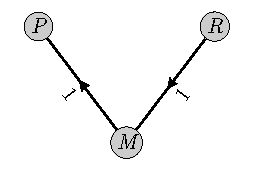
\includegraphics{comparisons/comparison-network-poorer}
    \end{center}

    \begin{parts}
        \part Let $\tilde \phi = \kappa_1 \phi$. Compute the social externality matrix $L$.

        \begin{solution}
        
            $G = \begin{pmatrix}
                0 & 0 & 0 \\ 1 & 0 & 0 \\ 0 & 1 & 0
            \end{pmatrix}$, 
            %
            $G^2 = \begin{pmatrix}
                0 & 0 & 0 \\ 0 & 0 & 0 \\ 1 & 0 & 0
            \end{pmatrix}$,
            %
            $G^3 = G^4 = \cdots = 0 \in \mathbb{R}^{3 \times 3}$

            Hence,

            $L = \sum_{i=1}^\infty \phi^i G^i = \begin{pmatrix}
                0 & 0 & 0 \\ \tilde \phi & 0 & 0 \\ \tilde \phi^2 & \tilde \phi & 0
            \end{pmatrix}$
        \end{solution}
        
        \uplevel{Recall that $\vec h = \kappa_2 \sum_{i = 0}^\infty (\tilde \phi G)^i \vec y$.}

        \part Compute $\frac{\partial}{\partial y^R} h_P$.

        \begin{solution}
            \begin{itemize}
                \item Note that $\sum_{i = 0}^\infty (\tilde \phi G)^i = I + L$
                \item Thus $\frac{\partial}{\partial y^R} h_P = \kappa_2 L_{PR}$ where $L_{PR}$ is the $(P, R)$ entry of the social externality matrix $L$.
                \item $L_{PR} = 0$ (from above)
            \end{itemize}
        \end{solution}

        \part Interpret this result and discuss its relevance.

        \begin{solution}
            \begin{itemize}
                \item $L_{ij}$ is the externality that $j$ exerts on $i$. It is positive, if $\phi > 0$ and if $i$ cares about $j$'s house (directly or indirectly).

                \item If $j$'s income goes up, and $j$ exerts an externality on $i$, then $i$ will spend more on housing (and less on consumption).
        
                \item Such behavior is well-documented empirically. It can help explain why household debt has increased so much between 1980 and 2007.
            \end{itemize}
        \end{solution}
    \end{parts}